\documentclass[10pt,twocolumn]{article}
\newcommand{\PaperShortTitle}{Measuring Coding-Agent Context Residency}
\usepackage{../paperstyle}

\title{\vspace{-1.2em}\textbf{Tokens Are Multiplied by Turns:}\\
\Large Measuring Context Residency, Reuse, and Reducibility in Coding Agents}
\author{Ankit\\\small\repo}
\date{}

\begin{document}
\maketitle
\thispagestyle{fancy}

\begin{abstract}
Token counts understate the cost of tool-using language-model agents.  An input admitted on turn $a$
can remain in the prompt and be processed again on every later turn, so its effective burden is its
length multiplied by its remaining lifetime.  We call this burden \emph{context residency} and its
unit the \tokensturn.  We develop an accounting method that reconstructs real API calls from
multi-record transcripts, separates context occupancy from provider-priced cost, attributes resident
content to prompt and tool channels, and distinguishes retrospective opportunity from interventions
that can be applied prospectively.  Three complementary design-partner datasets ground the analysis:
an exploratory archive of approximately 168 Claude Code sessions, a preregistered and stratified
50-task Django/SWE-bench-style observation corpus, and 60 single-window coding sessions used for
prefix decomposition.  Cache re-reads account for 96\% of occupancy in the exploratory archive.  In
the 60-session decomposition, the fixed system/tool/injected prefix accounts for 73.0\% of resident
input \tokensturns, while retained hidden thinking accounts for an estimated 11.3\%.  In the frozen
50-task corpus, 21.3\% of fully measured read tokens are retrospectively identifiable exploration
candidates and 51.0\% form a broader ceiling when search/listing output is included; run-bootstrap
95\% intervals are 15.9--27.0\% and 43.7--58.8\%, respectively.  These are candidate masses, not
guaranteed savings.  A sequence of negative results---zero voluntary use of a semantic read surface,
graph retrieval that fails a joint recall--budget gate, and eager discovery packets that increase
pooled input 55.6\%---shows why token compression ratios alone are insufficient.  The resulting
measurement discipline motivates cache-aware admission and lifetime control, evaluated separately
in the companion systems paper.
\end{abstract}

\section{Introduction}

Coding agents repeatedly call a language model while reading files, searching a repository, editing
code, running tests, and inspecting failures.  The prompt on turn $t$ is usually not a fresh message;
it contains a fixed system prefix, tool definitions, injected instructions, and much of the prior
trajectory.  A 2,000-token tool result admitted early in a 50-call session can therefore create close
to 100,000 input \tokensturns even if it is never read again by the human.  Conversely, removing 2,000
tokens from the last request saves almost nothing.  The relevant question is not merely \emph{how
many tokens can be shortened?} but \emph{which tokens are present, for how many future requests, and
under which cache state?}

This distinction is easy to lose because three denominators coexist.  First, a context window limits
the number of tokens resident on one request.  Second, cumulative input workload sums that occupancy
over an agent trajectory.  Third, an API bill weights uncached input, cache reads, cache writes, and
output differently.  A transformation can improve the first quantity while worsening the third if it
invalidates a cheap cached prefix and creates an expensive rewrite.  Under the one-hour cache tier
used in our experiments, a write is priced at $2\times$ base input while a hit is $0.1\times$
\cite{anthropicPromptCaching}.  Thus even a semantically safe deletion may have negative short-run
economic value.

The literature provides strong solutions to adjacent problems.  Prompt-compression methods remove
lexical units or learn compact representations \cite{jiang2023llmlingua,jiang2024longllmlingua,
pan2024llmlingua2,ge2024icae,xu2024recomp}.  Agent-memory systems page, summarize, or actively compact
history \cite{packer2023memgpt,liu2026cat,verma2026focus,zhang2026autocompact}.  Repository retrievers
select code using similarity or graphs \cite{zhang2023repocoder,liu2024graphcoder,chen2025locagent}.
Serving systems reuse and schedule KV state \cite{kwon2023pagedattention,zheng2024sglang,
gim2024promptcache,srivatsa2024preble}.  These methods establish that less or better-selected context
can preserve or improve task quality.  They do not by themselves tell a client-side coding-agent
runtime which admitted object is responsible for cumulative workload, whether its deletion is known
safe at decision time, or whether the cache-write penalty dominates future read savings.

This paper supplies that missing empirical layer.  It makes four contributions:

\begin{enumerate}
  \item We define a dual ledger for \emph{occupancy} and \emph{economics}, centered on the
  \tokensturn and an object-level residency graph.
  \item We provide a trace-reconstruction method that merges records belonging to one API request,
  excludes sidechains from main-trajectory totals, and explicitly separates measured from estimated
  token classes.
  \item We quantify where coding-agent context accumulates using complementary observational and
  controlled corpora, including a preregistered 50-task sample and task-cluster uncertainty.
  \item We report the failed mechanisms, not only the surviving story.  Those results reveal three
  recurring errors: confusing retrospective labels with prospective policies, optimizing bytes
  instead of \tokensturns, and ignoring cache rewrite economics.
\end{enumerate}

All code, protocols, aggregate artifacts, gateway logs used by the companion paper, and scripts that
regenerate the figures and tables are in the repository \cite{contextruntime2026}.  The work is a
single-provider, single-primary-repository design-partner study.  Its measurements are evidence for
mechanism and experimental design, not a market-wide prevalence estimate.

\section{Accounting Model}

\subsection{From token counts to residency}

Let $P_t$ denote the model-visible input on API call $t$:
\begin{equation}
P_t = U_t + R_t + W_t,
\end{equation}
where $U_t$ is uncached input, $R_t$ is cache-read input, and $W_t$ is cache-creation input.  The
cumulative input workload of a trajectory with $T$ calls is
\begin{equation}
\mathcal{W}=\sum_{t=1}^{T} P_t.
\end{equation}
The unit of $\mathcal{W}$ is the \tokensturn.  It is an implementation-facing measure of context
work, not a claim about the internal floating-point operations of a proprietary model.

For an object $i$ with size $s_i$, admitted at call $a_i$ and last resident at call $d_i$, its idealized
residency burden is
\begin{equation}
\mathcal{R}_i=s_i(d_i-a_i+1).
\end{equation}
An object may be a tool schema, system-prompt segment, file read, shell output, assistant thought, or
edit payload.  A context-residency graph records object lineage, re-delivery, supersession, and the
calls over which the object remains resident.  The graph makes explicit why admission and retirement
are dual operations: admission controls $s_i$ and $a_i$; retirement controls $d_i$.

\subsection{The economic ledger}

Provider billing is a weighted ledger rather than a token total.  For price profile
$\pi=(\alpha,\rho,\omega,\beta)$, we compute
\begin{equation}
\mathcal{B}_{\pi}=\sum_t(\alpha U_t+\rho R_t+\omega W_t+\beta O_t),
\end{equation}
where $O_t$ is model output.  The experiments in the companion paper use
$(1,0.1,2,5)$, matching the one-hour cache-write, cache-hit, and output ratios of the selected model
at collection time.  We retain the vector $(U,R,W,O)$ in every artifact so that results can be
repriced rather than frozen to one vendor schedule.

The two ledgers answer different questions.  $\mathcal{W}$ approximates context-window pressure and
input processing across the trajectory.  $\mathcal{B}_{\pi}$ answers what the observed usage would
cost under $\pi$.  A policy is not declared economically beneficial merely because it reduces
$\mathcal{W}$.

\subsection{Prospective and retrospective knowledge}

At analysis time, future events are visible.  At runtime, they are not.  We therefore distinguish:

\begin{itemize}
  \item \textbf{Prospective controls} use only information available before sending the current
  request: content type, age, cache state, known supersession, and configured tool permissions.
  \item \textbf{Retrospective ceilings} may use the remainder of the completed trajectory to ask what
  would have been removable by an oracle.
\end{itemize}

This distinction is central.  A file read that is never followed by an edit to the same path is a
retrospective exploration candidate.  The observation does not prove that the read was semantically
unnecessary for a later edit elsewhere, nor could a runtime have known its future role when the read
first arrived.  We use the word \emph{ceiling} whenever either limitation applies.

\section{Relation to Prior Research}

The most useful comparison is by intervention boundary rather than by headline compression ratio.
Table~\ref{tab:landscape} summarizes the boundary and the remaining gap.

\begin{table*}[t]
\centering
\caption{Research landscape and the distinct question addressed here. ``Cache-aware'' means the
decision objective explicitly includes prefix validity or provider-tier economics, not merely that
the implementation can benefit from a cache.}
\label{tab:landscape}
\small
\begin{tabularx}{\textwidth}{p{0.16\textwidth}p{0.23\textwidth}p{0.20\textwidth}cX}
\toprule
Family & Representative work & Primary unit optimized & Cache-aware & Boundary relative to this work \\
\midrule
Prompt compression & LLMLingua, LongLLMLingua, LLMLingua-2, RECOMP, ICAE
\cite{jiang2023llmlingua,jiang2024longllmlingua,pan2024llmlingua2,xu2024recomp,ge2024icae}
& tokens in one supplied prompt or retrieved document & usually no & Strong evidence that prompts can
be compressed; limited accounting for repeated admission over an evolving agent trajectory. \\
Agent memory / compaction & MemGPT, CAT, Focus, AutoCompact
\cite{packer2023memgpt,liu2026cat,verma2026focus,zhang2026autocompact}
& remembered semantics and bounded trajectory state & partial & Closest semantic relatives.  Our
focus is measured object lifetime, fail-open mutation, and cache-priced break-even behavior. \\
Repository retrieval & RepoCoder, GraphCoder, LocAgent
\cite{zhang2023repocoder,liu2024graphcoder,chen2025locagent}
& relevance, localization, completion or issue-resolution accuracy & no & Better retrieval can reduce
context, but relevance/accuracy does not imply a positive whole-session token or dollar return. \\
Tool discovery & Re-Invoke, ToolRerank, MCP-Zero
\cite{chen2024reinvoke,zheng2024toolrerank,fei2025mcpzero}
& tool recall/ranking and selected-schema count & rarely & Directly supports deferred admission.  We
measure schema residency in a live coding client and expose a proxy-specific de-deferral failure. \\
KV-cache serving & vLLM, SGLang, Prompt Cache, ChunkAttention, Preble
\cite{kwon2023pagedattention,zheng2024sglang,gim2024promptcache,ye2024chunkattention,srivatsa2024preble}
& server memory, throughput, TTFT, prefix reuse & yes & Server-side systems decide placement and
reuse; this work observes a black-box API and decides whether client-side prompt mutation pays. \\
Agent prompt caching & Don't Break the Cache, CAPC, keepalive economics
\cite{lumer2026cache,song2026capc,khailo2026keepalive}
& provider-priced reuse over multi-turn workloads & yes & Concurrent and highly complementary.
We add content-object attribution, coding-agent mutation safety, and a pre-registered intervention
lineage from failed mechanisms to live results. \\
\bottomrule
\end{tabularx}
\end{table*}

\subsection{Prompt compression and long-context behavior}

LLMLingua reports up to $20\times$ compression with little loss on several prompting scenarios;
LongLLMLingua targets retrieval ordering and long-context position bias; LLMLingua-2 reframes
task-agnostic compression as token classification \cite{jiang2023llmlingua,jiang2024longllmlingua,
pan2024llmlingua2}.  RECOMP trains extractive and abstractive compressors for retrieved documents,
including selective empty augmentation \cite{xu2024recomp}.  Gist tokens and ICAE learn compact
latent prompt representations \cite{mu2023gist,ge2024icae}.  Li et al. provide a broader taxonomy of
hard and soft prompt compression \cite{li2025survey}.

These works demonstrate that redundancy can be removed, but compression quality is not the only
constraint in an agent loop.  The compressed artifact can remain resident for dozens of future calls;
a query-dependent rewrite can also break a stable cache prefix.  Moreover, long advertised windows do
not guarantee uniform use of evidence: ``lost in the middle'' behavior and RULER both motivate
evaluating effective, rather than nominal, context \cite{liu2024lost,hsieh2024ruler}.  Our
contribution is not a new linguistic compressor.  It identifies the objects and time intervals for
which a compressor, deferrer, or deleter could have system-level leverage.

\subsection{Agent memory and active compaction}

MemGPT treats context as virtual memory and exposes tiered movement to the model
\cite{packer2023memgpt}.  Recent coding-agent systems bring compaction inside the trajectory.  CAT
uses a structured workspace and model-called context maintenance, reporting 57.6\% solved on
SWE-bench Verified \cite{liu2026cat}; Focus reports 22.7\% token reduction on five SWE-bench Lite
instances at equal 3/5 success \cite{verma2026focus}; AutoCompact learns when to compact from
supervised and reinforcement-learning signals \cite{zhang2026autocompact}.  The broader memory
literature spans storage, retrieval, reflection, and update operations \cite{zhang2025memorysurvey}.

Our results reinforce this direction but also show why the controller matters.  Voluntary adoption
can be zero, eager replacement packets can increase whole-session workload, and unaligned deletion can
turn cheap reads into expensive writes.  We therefore treat semantic policy, object safety, and cache
economics as separable gates.

\subsection{Code retrieval and graph context}

SWE-bench established repository-scale issue resolution as a long-context, environment-interaction
problem \cite{jimenez2024swebench}.  SWE-agent showed that the agent-computer interface materially
changes performance \cite{yang2024sweagent}, while Agentless demonstrated the strength and low cost of
a simple localization--repair--validation pipeline \cite{xia2025agentless}.  RepoCoder iterates
similarity retrieval and generation; GraphCoder and LocAgent use structural graphs for completion or
localization \cite{zhang2023repocoder,liu2024graphcoder,chen2025locagent}.

Those results motivate our own graph experiments but do not guarantee a token win.  A graph may find
useful code yet require an anchor the issue text does not provide, or may spend more tokens to achieve
the necessary support recall.  We report both failures below.  The conclusion is scoped: graphs are
valuable representations and can improve localization; they did not clear our joint recall--budget
gate as the primary saving mechanism in this Django sample.

\subsection{Caching and tool admission}

PagedAttention reduces KV-memory fragmentation, SGLang's RadixAttention reuses shared prefixes, and
Prompt Cache makes reusable prompt modules explicit \cite{kwon2023pagedattention,zheng2024sglang,
gim2024promptcache}.  ChunkAttention shares prefix chunks; RAGCache and CacheBlend reuse knowledge
state; Preble schedules shared prompts across devices; Parrot exposes application-level dataflow
\cite{ye2024chunkattention,jin2024ragcache,yao2025cacheblend,srivatsa2024preble,lin2024parrot}.
These optimize an inference service that can see or control KV state.  A client of a proprietary API
instead observes billed cache reads and writes and can only shape request content and timing.

Tool retrieval attacks a particularly expensive fixed prefix.  Re-Invoke and ToolRerank improve tool
retrieval; MCP-Zero constructs a task-specific toolchain \cite{chen2024reinvoke,zheng2024toolrerank,
fei2025mcpzero}.  Provider tool search similarly defers schemas and explicitly warns that definitions
and accumulated results consume context \cite{anthropicAdvancedTools,anthropicToolContext}.  Our
measurement places this idea inside an end-to-end cost ledger and finds that a custom base URL can
disable the client's normal deferral behavior \cite{anthropicMCP}---an interaction large enough to
invalidate an otherwise well-designed experiment.

\section{Data and Measurement Design}

\subsection{Three complementary datasets}

No single dataset supports every claim.  We therefore use three layers and preserve their evidence
grades.

\textbf{D1: exploratory design-partner archive.}  Approximately 168 personal Claude Code sessions
and roughly 170,000 logged requests were profiled to locate large mechanisms.  This convenience sample
includes varied interactive work and is used only for structural observations such as cache-read
dominance, rebuild causes, aged-result occupancy, and concentration.  The private raw archive is not
redistributed.  Aggregate reports and the analysis code are retained in the repository.  We do not
use D1 for population inference.

\textbf{D2: frozen observation corpus.}  Fifty Django tasks were selected from the 231 Django
instances in SWE-bench Verified using a SHA-256 rank fixed before collection.  The design balances
five gold-patch shape strata---one-line, small, medium, large, and multi-file---at ten tasks each.
Selection and execution order use separate namespaces.  Each run starts from a pinned base commit in
an isolated worktree; failures remain in place.  The task run, not an individual read, is the sampling
unit.  Forty-seven of 50 runs satisfy every canonical admission check.  All 50 are retained, and 49
contain substantive reads and edits.  Official grading resolves 40/50 patches.

\textbf{D3: prefix decomposition set.}  Sixty single-window Django coding sessions, averaging 49.5
real API calls and 42,451 startup tokens, support a channel-level decomposition of cumulative input.
The system prompt is not directly visible in transcripts; its mass is inferred as the residual needed
to reconcile the first-call provider usage after observed tool and injected segments are counted.
Consequently the fixed-prefix share has a documented hard lower bound of 66.9\%, while the best
estimate is 73.0\%.  Invisible retained thinking is estimated as output tokens minus visible output.

The companion systems paper adds B6--B8 live and replay datasets.  Keeping those results separate
prevents intervention outcomes from redefining the measurement taxonomy that selected them.

\subsection{Trace reconstruction}

Claude Code can record one API response on multiple transcript lines that share a \texttt{requestId};
each line can repeat the same usage block.  Treating lines as calls inflated both the turn axis and
summed usage by about $1.9\times$ in an early harness.  The corrected parser groups records by
\texttt{requestId}, merges their content, and counts the usage once.  Main-trajectory analysis follows
parent lineage and excludes sidechains unless a study explicitly declares them in scope.  The parser
then exactly reproduces the CLI-reported usage on validation sessions.

This correction is more than bookkeeping.  Residency grows with the number of future calls, so an
inflated call index biases the apparent benefit of late retirement.  We keep the original corrected
notes and commit history to make this failure auditable.

\subsection{Read-role evidence}

The observation runtime records pre- and post-tool events, mutations, virtual working directory, and
causal read-to-edit links.  A run is canonical only when calls reconcile, capture errors and pending
tools are zero, schemas match, provenance is complete, and no sequential fallback was required.
Across D2, 538 of 589 classified reads (91.3\%) have fully attributed text-token weights.  The
remaining 51 are composite or multipath ambiguities; no multimodal read enters the token headline.
Every edit-precondition link uses actual event linkage rather than temporal proximity, and 76.6\% are
at causal distance one.

Roles are intentionally conservative: 18.8\% of read events are edit preconditions, 12.2\%
exploration, 1.7\% verification, and 67.2\% unknown.  Much of ``unknown'' is search output that the
runtime refuses to promote to a file-specific role.  Bash coverage is not certified complete and the
\texttt{config\_required} category is unexercised.  Those scope gaps remain exclusions rather than
being relabeled to improve the opportunity estimate.

\subsection{Estimands and uncertainty}

For D2 we report the token-weighted micro ratio, task-level macro mean and median, equal-stratum mean,
and per-stratum values.  The micro estimand answers where measured tokens occur in this balanced
design; it is not an estimate of natural production traffic.  We resample task runs, not read events,
100,000 times to obtain percentile bootstrap intervals for the two opportunity ratios.  The bootstrap
quantifies run-to-run variation inside this corpus; it does not repair single-repository or
single-client external-validity limits.

\begin{figure*}[t]
\centering
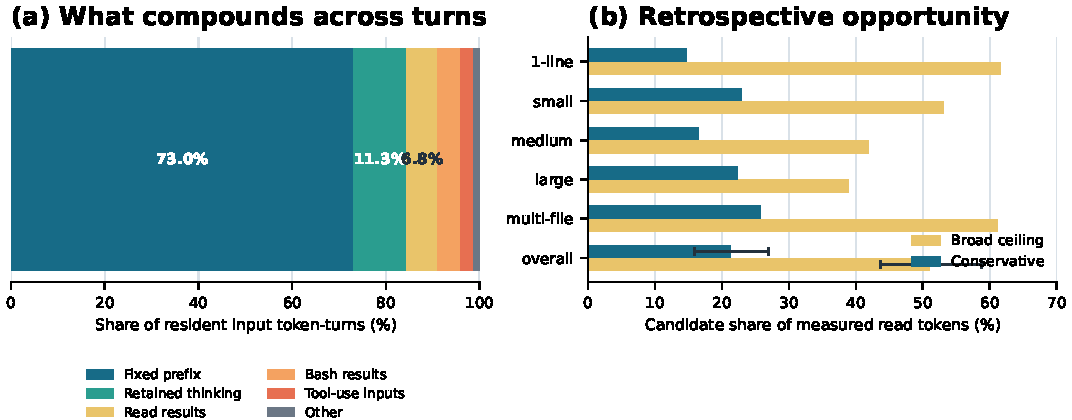
\includegraphics[width=\textwidth]{../figures/measurement_overview.pdf}
\caption{Measured context structure.  (a) Channel decomposition across 60 single-window Django
sessions; retained thinking is estimated and the fixed-prefix estimate has a 66.9\% hard lower bound.
(b) Candidate read-token mass across five balanced fix-shape strata and overall in the frozen 50-run
corpus.  Overall whiskers are task-run bootstrap 95\% intervals.  The broad ceiling adds
search/listing output to retrospective exploration candidates; neither bar is a guaranteed saving.}
\label{fig:measurement}
\end{figure*}

\section{Results}

\subsection{The repeated prefix dominates}

In D1, cache re-reads form 96\% of context occupancy.  Eighty-two percent of cache-write tokens are
prefix rebuilds rather than newly appended content; approximately 64\% of the rebuild mass is
attributed to unavoidable idle-TTL expiry and 24\% to addressable client behavior.  Tool results that
remain resident for more than 50 turns account for about 23\% of occupancy.  Exact hash-identical
re-delivery is only 2.4\%, model-switch churn 2.7\%, and rewrite amplification 1.3$\times$.  The top 20
sessions contribute 74\% of occupancy.  These exploratory values establish concentration and
mechanism, not cross-user prevalence.

D3 explains why naive cleanup underperforms.  Figure~\ref{fig:measurement}(a) assigns 73.0\% of input
\tokensturns to the fixed system/tool/injected prefix.  Retained hidden thinking contributes an
estimated 11.3\%, file-read results 6.8\%, Bash results 4.9\%, and tool-use inputs 2.7\%.  Polling
turns account for only 0.5\% on average.  Same-path file refreshes add about 2,103 tokens per session,
roughly 1\% of cumulative input after their remaining lifetime is considered.  Edit
\texttt{old\_string} duplication of a resident read is zero in this sample.

The economic ledger changes the composition but not the priority.  In these sessions, cache reads are
97.6\% of input tokens yet 60.8\% of price-weighted cost; cache writes are 1.8\% of input but 22.4\%
of cost; output is about 0.5\% of tokens and 16.7\% of cost.  A prefix rewrite can therefore dominate
the savings from removing a modest result.  The strongest lever must reduce a large early object while
preserving or deliberately rebuilding the cache.

\claimbox{\textbf{Finding 1 (\observed).}  Coding-agent context is predominantly a lifetime problem.
The fixed prefix is multiplied across calls, and provider cache writes make poorly timed mutation
economically discontinuous.}

\subsection{Read-level opportunity is substantial but not directly actionable}

D2 contains 246,686 fully measured read tokens.  The conservative bucket contains 52,535 tokens
(21.3\%): file reads retrospectively labeled as exploration because the same path is not later
mutated.  The broader ceiling adds 73,360 search/listing tokens, reaching 125,895 tokens (51.0\%).
The remaining mass comprises 70,726 edit-precondition tokens (28.7\%), 44,610 unresolved tokens
(18.1\%), and 5,455 verification tokens (2.2\%).

The run-bootstrap 95\% interval is 15.9--27.0\% for the conservative ratio and 43.7--58.8\% for the
broad ratio.  Reweighting supports the structural conclusion: conservative micro/macro-mean/
macro-median/equal-stratum estimates are 21.3/17.3/9.6/20.4\%; broad estimates are
51.0/47.4/44.7/51.3\%.  The conservative opportunity is right-skewed---a quarter of tasks contain no
confident exploration candidates and only 25/50 exceed 10\%.  The broad opportunity is more stable:
47/50 tasks exceed 10\%, and every stratum lies between 38.9\% and 61.6\%.

These ratios are deliberately called ceilings.  Search/listing content is identifiable prospectively
by type, but a safe summary still needs to preserve filenames, matches, and evidence used later.
Exploration is known only retrospectively and same-path non-mutation does not imply semantic
irrelevance.  The gap between candidate mass and realized savings must be closed by an intervention
with task-quality checks.

\claimbox{\textbf{Finding 2 (\observed ceiling).}  Half of measured read tokens fall into a broad
reduction-candidate set, but only 29.7 percentage points are type-identifiable prospectively.  The
remaining 21.3 points depend on future knowledge and cannot be advertised as safe live savings.}

\subsection{Four mechanisms fail for four different reasons}

Table~\ref{tab:negative} collects the program's negative and boundary results.  They are important
because each would look promising under a narrower denominator.

\begin{table*}[t]
\centering
\caption{Mechanism-screening ledger.  Gates were written before the corresponding confirmatory run
where noted.  ``Closed'' means closed as a primary token-saving lever in this environment, not a claim
that the representation or idea is universally useless.}
\label{tab:negative}
\small
\begin{tabularx}{\textwidth}{p{0.16\textwidth}p{0.21\textwidth}p{0.23\textwidth}p{0.15\textwidth}X}
\toprule
Mechanism & Attractive local metric & Whole-system evidence & Evidence type & Decision / lesson \\
\midrule
Search-output compaction & 12.1\% fewer search-output tokens in prior replay & Direct saving only
0.028--0.048\% of total live input; call count explains 98.8\% of total variation & 40-arm live study,
57 completed runs across all arms & Safe locally, too small in the repeated-prefix denominator. \\
Semantic read surface & Budget-correct symbol bundles; forced calls resolve & 0/11 spontaneous uses
across two delivered advisory prompts & 11 live runs, 6 tasks & Advisory adoption closed; a usable
mechanism without adoption has zero product effect. \\
Graph-first context & At 2,048 tokens, oracle-anchored bundle is 41\% of native exploration & Problem
text anchors reach 0/14 edited symbols; task-graph budgets never clear recall and token gates together
& Offline G1 (14 edits) and G2 (3 tasks) & Graph is a relevance representation, not automatically a
token-saving policy. \\
Discovery call collapse & Offline evidence-gated oracle removes 13.1\% of calls at $>$96\% evidence
retention & Forced eager packets raise mean input 71.6\% and pooled input 55.6\% & 3 enforced live
tasks after offline oracle & Iterative multi-kilobyte packets remain resident; local call reduction
does not imply \tokensturn reduction. \\
\bottomrule
\end{tabularx}
\end{table*}

\textbf{Search compression optimizes a small slice.}  A transparent reducer preserved evidence and
removed 12.1\% of search-output tokens in replay.  In live replicated runs, however, the directly
removed mass was only 935--1,807 tokens per session, 0.028--0.048\% of cumulative input.  Across 57
completed trajectories, total input was 98.8\% explained by the number of calls.  The treatment arms
made slightly more calls, so whole-session totals rose despite genuine per-result compression.  The
mechanism was safe but not material.

\textbf{A correct interface can have zero adoption.}  A SemanticFS server indexed 43,241 Django
symbols, resolved natural names, and returned budget-valid bundles.  Two independently written system
prompts asked the agent to use the surface.  Delivery was logged and forced calls worked, yet voluntary
adoption was 0/11.  Repository issues often provided concrete paths or tracebacks that competed with a
new abstract interface.  We closed advisory-only adoption rather than counting potential bundle
savings as realized.

\textbf{Graph recall and token budget form a joint gate.}  In G1, a problem-statement anchor reached
none of 14 edited symbols.  Supplying the edited symbol as an oracle anchor improved symbol recall to
0.857 and edit-line/body recall to 0.571 at a 2,048-token budget; the bundle was 41\% of native
exploration tokens.  The result is compression conditional on already knowing the target.  In G2, a
task-relevance graph had a budget-free support ceiling of 0.739, but at 1,024 tokens its 0.137 recall
gain missed the 0.15 gate; at 2,048 and 4,096 tokens the gain cleared 0.15 only by spending 49\% and
195\% more tokens than lexical retrieval.  No budget cleared both gates.  This does not contradict
LocAgent or GraphCoder, whose target is localization/completion quality rather than our joint
whole-session saving criterion.

\textbf{An offline call oracle can reverse live.}  Discovery accounts for 50.4\% of calls in a
60-session analysis.  An evidence-gated oracle suggested 13.1\% of all calls could collapse while
retaining 97.1\% of next-action evidence, 100\% of edit-target evidence, and 96.3\% of edit-region
evidence.  A live executor then enforced the replacement.  Agents used it as a search engine, making
15--16 iterative calls per session; each eager multi-kilobyte packet stayed resident.  Across three
tasks, input rose 11.5\%, 39.5\%, and 163.8\% (mean +71.6\%, pooled +55.6\%).  The enforcement run
converted cheap probes into expensive resident packets.  We closed the eager-packet design rather
than add a learned retriever to rescue the hypothesis.

\claimbox{\textbf{Finding 3.}  Compression ratio, retrieval recall, adoption, and cache economics are
independent gates.  Passing any one does not license an end-to-end efficiency claim.}

\section{What the Field Has Established---and the Remaining Story}

The literature and our evidence now support a cleaner research story than ``agents use too many
tokens.''

\textbf{Established: content can be compressed.}  Textual and latent compressors achieve large
ratios on QA, summarization, and long-context tasks \cite{jiang2023llmlingua,jiang2024longllmlingua,
pan2024llmlingua2,ge2024icae,xu2024recomp}.  This motivates a compression operator but not where to
apply it in a coding trajectory.

\textbf{Established: managed memory can preserve long-horizon capability.}  Virtual memory,
structured workspaces, and agent-controlled compaction improve bounded-context operation
\cite{packer2023memgpt,liu2026cat,verma2026focus,zhang2026autocompact}.  This motivates lifetime
control but leaves the timing and billing objective open.

\textbf{Established: repository structure improves retrieval in some tasks.}  Iterative and graph
retrieval improve completion or localization \cite{zhang2023repocoder,liu2024graphcoder,
chen2025locagent}.  Our evidence says the quality objective and a token-saving objective must be
evaluated separately, especially when anchors are unknown.

\textbf{Established: prefix reuse is a systems primitive.}  Serving systems obtain large throughput
or latency gains by reusing KV state \cite{kwon2023pagedattention,zheng2024sglang,gim2024promptcache,
ye2024chunkattention,srivatsa2024preble}.  Recent API-level work shows that cache strategy materially
changes multi-turn cost \cite{lumer2026cache,song2026capc,khailo2026keepalive}.  This motivates a
cache-aware controller rather than deletion at a fixed token threshold.

\textbf{The gap: causal, economic object lifetime in real coding agents.}  The missing layer connects
what an object means, how long it will remain, whether it can be changed safely, and what that change
does to a black-box provider cache.  Our measurement results identify fixed-prefix admission as the
largest prospective lever, old tool/thinking state as a tail lever, and cache-aligned timing as the
condition that makes deletion economically sane.  The companion paper turns that map into a runtime
and tests it live.

\section{Implications for Evaluation and Design}

\subsection{Report a claim ladder}

Every efficiency number should name its rung:

\begin{enumerate}
  \item \textbf{Candidate mass}: tokens matching a retrospective or type-based rule.
  \item \textbf{Counterfactual opportunity}: replay under an explicit behavior/cache model.
  \item \textbf{Live context reduction}: observed cumulative input under an intervention.
  \item \textbf{Live economic reduction}: observed or transparently repriced billing components.
  \item \textbf{Quality-preserving reduction}: the above with objective task evaluation and a frozen
  acceptance rule.
\end{enumerate}

Moving upward requires new evidence; ratios must not be relabeled.  In particular, B7's roughly 60\%
pooled giant-session result in the companion paper remains modeled even though its cache model is
validated elsewhere.

\subsection{Treat negative results as mechanism localization}

The failed sequence was not wasted effort.  Zero adoption identifies a policy-interface problem.
Graph failure separates retrieval relevance from economic value.  Search compression shows that a
safe local reducer can be immaterial in the global denominator.  Eager packets expose residence time
as the hidden multiplier.  Each result removes a branch from the causal story and motivates the final
architecture more strongly than a post-hoc collection of favorable ablations.

\subsection{Optimize admission before sophisticated memory}

The fixed prefix contributes 73.0\% of observed input \tokensturns, and tool definitions can be
deferred or disallowed before the first request.  Old results matter primarily in long-tail sessions.
Thus a robust deployment should begin with a prefix audit, remove servers and schemas that cannot be
used, retain a small always-on core, and then add lifetime policies.  Provider guidance now recommends
the same layered decomposition---tool search for definitions, programmatic calls for round trips,
prompt caching for stable content, and context editing for old results \cite{anthropicToolContext}.
Our contribution is to make the ordering empirical and auditable.

\section{Threats to Validity}

\textbf{External validity.}  The controlled corpora use Django and Claude Code.  Django is large and
real, and SWE-bench tasks require repository navigation, but languages, agents, tools, models, and
provider caches differ.  D1 is a single-user convenience sample.  We label all results
design-partner evidence and do not extrapolate prevalence.

\textbf{Construct validity.}  $\mathcal{W}$ measures billed/model-visible input, not energy, latency,
or exact attention FLOPs.  Hidden thinking is estimated.  The fixed-prefix residual is bounded but
not fully observable.  The economic ledger uses a stated price profile and should be repriced when
provider terms change.

\textbf{Causal validity.}  Retrospective same-path labels do not prove semantic dispensability.
Replays hold the recorded trajectory fixed and cannot capture behavioral adaptation unless followed
by a live experiment.  That is why candidate and modeled quantities remain explicitly below live
claims.

\textbf{Sampling and uncertainty.}  The 50-task corpus is balanced by fix shape rather than sampled
in natural traffic proportions.  Bootstrap intervals contain only 50 task units.  G1/G2 and the eager
executor use small diagnostic samples and support scoped mechanism decisions, not universal nulls.

\textbf{Instrumentation.}  Raw private design-partner transcripts cannot be released.  The frozen
controlled artifacts, protocols, hashes, request-merging parser, and derived summaries are released.
An early request-counting error demonstrates that instrumentation bugs are plausible; preserving the
correction and reconciling to CLI totals reduces, but cannot eliminate, this risk.

\section{Conclusion}

The effective cost of coding-agent context is governed by length, lifetime, and cache state.  In our
design-partner measurements, repeated fixed content dominates cumulative input, and read-level
candidate mass substantially overstates immediately realizable savings.  Negative experiments show
why: agents may ignore a new interface, graphs may miss a joint recall--budget gate, a locally small
reducer may disappear in the whole-session denominator, and eager replacement packets can remain
resident long enough to reverse the expected benefit.  A defensible efficiency claim must therefore
connect object semantics to future calls and cache economics, then survive a live quality-gated test.
The companion paper evaluates that systems path.

\section*{Artifact and Reproducibility Note}

The repository contains the frozen task plan, observation protocols, aggregate artifacts, mechanism
findings, analysis code, and the exact script that regenerates this paper's figure and bootstrap
intervals.  Run \texttt{python3 papers/scripts/generate\_assets.py} from the repository root, then
build this source with \texttt{latexmk -pdf main.tex}.  No paid model calls are needed to reproduce
the reported analyses.

\bibliographystyle{plain}
\bibliography{../references}

\end{document}
